\documentclass[12pt,a4paper,twoside,fleqn]{article}
\usepackage[utf8]{inputenc}
\usepackage[ngerman]{babel}
\usepackage[left=25mm, top=20mm, bottom=20mm, right=20mm]{geometry}
\usepackage{graphicx,overpic,color,marvosym,upgreek}
\usepackage{amssymb,multicol,amsmath}
%\usepackage{ifthen}
\usepackage{cancel}
\usepackage{float}
\usepackage{icomma} 


\begin{document}

\newcommand{\Vektor}[2]{\begin{pmatrix} #1 \\ #2 \end{pmatrix}}
\newcommand{\vektor}[3] {\begin{pmatrix} #1 \\ #2 \\ #3 \end{pmatrix}}
\newcommand{\umf}[1]{\qquad\left|#1\right.}
\newcommand{\uu}[1]{\underline{\underline{#1}}}

\renewcommand{\thepage}{Seite~\arabic{page}}
% \renewcommand{\thesection}{1.}
% \renewcommand{\thesubsection}{\arabic{subsection}}
\renewcommand{\baselinestretch}{1.2}

\renewcommand{\labelenumi}{{\bf\arabic{enumi}.)}}
\renewcommand{\labelenumii}{{\bf\alph{enumii})}}
\renewcommand{\labelenumiii}{{\bf\roman{enumiii})}}

\newcounter{column}
\renewcommand{\thecolumn}{{\bf\alph{column}\ }}
\newcommand{\labelcolumn}{{\bf\alph{column})\ \ \ }}
\setlength{\itemsep}{0pt}
\setlength{\mathindent}{0cm}
\newcounter{last}


\pagestyle{myheadings}
\markboth{\hfill Kurs: Orthogonalität und Produkte von Vektoren}%
{Kurs: Orthogonalität und Produkte von Vektoren\hfill}
\title{Orthogonalität und Produkte von Vektoren.\\\large{Ein Kurs
  zum selbständigen Lernen.}}
\author{Alexander Ruhri\\
  \small\texttt{a.ruhri@widarschule.de}\\
  \small Aktuelle Version unter \texttt{http://www.ruhri.net/}\\
  \small Lösungen: Tim Strunkheide}
\date{\small Version 0.4, Mai 2016}
% Todo: Lösungen
\maketitle
\section*{Vorbemerkungen}
Bitte beachten Sie beim Bearbeiten dieser Blätter, dass an geeigneten
Stellen Zusammenfassungen mit der ganzen Klasse durchgeführt
werden. Bitte machen Sie Ihren Lehrer darauf aufmerksam, wenn Sie das
Bedürfnis nach einer solchen Besprechung haben. 
\subsection*{Voraussetzungen}
Um mit den Inhalten des Kurses zurechtzukommen ist es notwendig,
dass Sie wissen, was ein Vektor ist, wie man die Länge eines Vektors
berechnet und die Parameterdarstellung von Geraden bereits gelernt
haben. Außerdem sollten Sie die Winkelfunktionen ($\sin, \cos$)
wiederholt haben.
\subsection*{Arbeitsweise}
Notieren Sie Ihre Rechnungen in einem Heft oder auf Blättern. Heben
Sie dabei Regeln optisch hervor und übertragen Sie diese nach
Überprüfung in ein eigenes Regelheft.
\tableofcontents
\part{Kurs}
\section{Orthogonale Vektoren}
Das Wort orthogonal leitet sich vom griechischen
$o\rho\theta o\varsigma$  (orthos)
„richtig, recht-“ und $\gamma\omega\nu\iota\alpha$ (gonia) „Ecke, Winkel“ ab
(vergl. \texttt{http://de.wikipedia.org/wiki/Orthogonalität}) und
bedeutet „rechtwinklig“. Wenn zwei Vektoren zueinander orthogonal
sind, kann man das in Zeichen so schreiben: $$\vec{a}\perp\vec{b}$$
\subsection{Orthogonale Vektoren finden}
\begin{enumerate}
\item Zeichnen Sie Pfeile der Vektoren in ein Koordinatensystem ein und
  finden Sie (gleich lange) zu ihnen orthogonale Vektoren. Zeichnen
  Sie die orthogonalen Vektoren vom gleichen Punkt ausgehend ein und
  geben Sie ihre Koordinaten an. 

  \begin{multicols}{4}
    \begin{enumerate}
    \item $\vec{a}=  
      \begin{pmatrix}
        0\\1
      \end{pmatrix}
      $
    \item $\vec{b}=  
      \begin{pmatrix}
        1\\1
      \end{pmatrix}
      $
    \item $\vec{c}=  
      \begin{pmatrix}
        3\\4
      \end{pmatrix}
      $
    \item $\vec{d}=  
      \begin{pmatrix}
        -7\\2
      \end{pmatrix}
      $
    \end{enumerate}
  \end{multicols}
\item Wenn Sie eine einfache Regel gefunden haben, mit der man gleich lange
  orthogonale Vektoren aus den Koordinaten des gegebenen Vektors  (im
  $\mathbb{R}^2$) bilden
  kann, dann formulieren und notieren Sie diese
  Regel. Ansonsten  versuchen Sie anhand weiterer Beispiele die Regel zu
  finden.
\item Beschreiben Sie das geometrische Objekt, das entsteht, wenn ein
  Punkt mit allen zu einem Vektor (im $\mathbb{R}^2$)  orthogonalen
  Vektoren (aller Längen), verschoben wird. 
\item Wie viele gleich
  lange orthogonale Vektoren hat ein Vektor im $\mathbb{R}^3$?
\item Beschreiben Sie das geometrische Objekt, das entsteht, wenn ein
  Punkt mit allen zu einem gegebenen Vektor orthogonalen Vektoren im
  $\mathbb{R}^3$ verschoben wird. Welches Objekt erhalten Sie, wenn
  die Vektoren alle gleich lang sind?
\item Finden Sie eine Methode, wie man zu einem gegebenen Vektor im
  $\mathbb{R}^3$ einen orthogonalen Vektor finden kann. Erweitern Sie
  dazu die Regel, die Sie in 2.) gefunden haben. (Tipp: Nehmen Sie die
  0 zu Hilfe.) Geben Sie orthogonale Vektoren zu den folgenden
  Vektoren an:
  
  \begin{multicols}{4}
    \begin{enumerate}
    \item $\vec{a}=  
      \begin{pmatrix}
        0\\1\\0
      \end{pmatrix}
      $
    \item $\vec{b}=  
      \begin{pmatrix}
        1\\1\\0
      \end{pmatrix}
      $
    \item $\vec{c}=  
      \begin{pmatrix}
        3\\0\\4
      \end{pmatrix}
      $
    \item $\vec{d}=  
      \begin{pmatrix}
        -7\\2\\1
      \end{pmatrix}
      $
    \end{enumerate}
  \end{multicols}
\item Untersuchen Sie, welche der folgenden Vektoren orthogonal
  zueinander sind:
  
  \begin{multicols}{3}
    \begin{enumerate}
    \item $\vec{a}=  
      \begin{pmatrix}
        0\\0\\1
      \end{pmatrix}
      $
    \item $\vec{b}=  
      \begin{pmatrix}
        -1\\0\\0
      \end{pmatrix}
      $
    \item $\vec{c}=  
      \begin{pmatrix}
        0\\-3\\0
      \end{pmatrix}
      $
     \end{enumerate}
  \end{multicols}
  
\end{enumerate}

\subsection{Vektoren auf Orthogonalität prüfen}
Als Test auf Orthogonalität zweier Vektoren kann man den Satz des
Pythagoras verwenden, denn er gilt nur in orthogonalen Dreiecken.
\vspace{.2cm}

\begin{minipage}[t]{.3\linewidth}
  \begin{overpic}[scale=.5,tics=10]%
    {pics/Dreieck}
    \put(-3,25){\scriptsize $\vec{b}$} \put(45,-3){\scriptsize
      $\vec{a}$} \put(45,30){\scriptsize $\vec{b}-\vec{a}$}
  \end{overpic}

\end{minipage}\hfill
\begin{minipage}[b]{.65\linewidth}
  Die beiden Vektoren in nebenstehender Skizze sind also genau dann
  orthogonal zueinander, wenn gilt: 
  $$|\vec{a}|^2 + |\vec{b}|^2 = |\vec{b} - \vec{a}|^2.$$
  Dabei ist
  $\vec{a}=
  \begin{pmatrix}
    a_1\\a_2
  \end{pmatrix}$ und
   $\vec{b}=
  \begin{pmatrix}
    b_1\\b_2
  \end{pmatrix}$ 
\end{minipage}
Wir betrachten nun die rechte und linke Seite der obigen Gleichung
(Satz des Pythagoras) getrennt voneinander.
Für die rechte Seite der Gleichung gilt nun:
\begin{align*}
|\vec{b} - \vec{a}|^2&=(b_1-a_1)^2 + (b_2-a_2)^2\\
\intertext{Anwenden der binomischen
  Formeln ergibt dann:}
|\vec{b} - \vec{a}|^2 &=(b_1^2-2b_1a_1 + a_1^2) + (b_2^2-2b_2a_2 + a_2^2)\\
\intertext{Durch Umstellen und Ausklammern erhalten wir:}
|\vec{b} - \vec{a}|^2 &= (a_1^2+ a_2^2)+ (b_1^2+b_2^2)
-2\cdot(a_1b_1+a_2b_2)\\
\intertext{Für die linke Seite der obigen Gleichung erhalten wir auf gleiche Weise:}
|\vec{a}|^2 + |\vec{b}|^2 &= (a_1^2+a_2^2) + (b_1^2+b_2^2)\\
\intertext{Insgesamt habe wir den Satz des Pythagoras folgendermaßen umgeformt:}
  |\vec{a}|^2 + |\vec{b}|^2 &= |\vec{b} - \vec{a}|^2 \\
 (a_1^2+ a_2^2)+ (b_1^2+b_2^2) &= (a_1^2+a_2^2) + (b_1^2+b_2^2)-2\cdot(a_1b_1+a_2b_2)
\end{align*}

Wenn wir linke und rechte Seite vergleichen, merken wir, dass der Satz
des Pythagoras nur dann gilt, wenn $ 2\cdot(a_1b_1+a_2b_2)=0$, also wenn
gilt: 
$$a_1b_1+a_2b_2=0$$
Insgesamt gilt also: $$\vec{a}\perp\vec{b} \Leftrightarrow a_1b_1+a_2b_2=0$$
\begin{enumerate}
\item Überprüfen Sie die von Ihnen gefundenen Vektoren mit dieser
  Regel auf Orthogonalität.
\item Überprüfen Sie folgende Paare von Vektoren auf Orthogonalität:
\begin{multicols}{4}
    \begin{enumerate}
    \item $ 
      \begin{pmatrix}
        2\\1
      \end{pmatrix};
      \begin{pmatrix}
        -6\\12
      \end{pmatrix}
      $
    \item $
      \begin{pmatrix}
        14\\-8
      \end{pmatrix} ;
      \begin{pmatrix}
        4\\7
      \end{pmatrix}
      $
    \item $
      \begin{pmatrix}
        -1\\-4
      \end{pmatrix} ;
      \begin{pmatrix}
        4\\1
      \end{pmatrix}
      $
    \item $
      \begin{pmatrix}
        7\\2
      \end{pmatrix};
      \begin{pmatrix}
        1\\-3,5
      \end{pmatrix}
      $
    \end{enumerate}
  \end{multicols}
\item Formulieren Sie diese Regel für den $\mathbb{R}^3$ indem Sie 
  $\vec{a}= \begin{pmatrix}
        a_1\\a_2\\a_3
      \end{pmatrix}$ und 
  $\vec{b}= \begin{pmatrix}
        b_1\\b_2\\b_3
      \end{pmatrix}$
verwenden.
\item Überprüfen Sie folgende Paare von dreidimensionalen Vektoren auf
  Orthogonalität:
\begin{multicols}{4}
    \begin{enumerate}
    \item $ 
      \begin{pmatrix}
        1\\0\\1
      \end{pmatrix};
      \begin{pmatrix}
        0\\1\\0
      \end{pmatrix}
      $
    \item $
      \begin{pmatrix}
        2\\3\\4
      \end{pmatrix} ;
      \begin{pmatrix}
        -4\\0\\2
      \end{pmatrix}
      $
    \item $
      \begin{pmatrix}
        1\\2\\3
      \end{pmatrix} ;
      \begin{pmatrix}
        2\\2\\-2
      \end{pmatrix}
      $
    \item $
      \begin{pmatrix}
        0\\0\\2
      \end{pmatrix};
      \begin{pmatrix}
        0\\-1\\1
      \end{pmatrix}
      $
    \end{enumerate}
  \end{multicols}
\item Finden Sie $a\in\mathbb{R}$, so dass die Vektoren orthogonal zueinander stehen.
  \begin{multicols}{4}
    \begin{enumerate}
    \item $ 
      \begin{pmatrix}
        3\\4\\1
      \end{pmatrix};
      \begin{pmatrix}
        -1\\2\\a
      \end{pmatrix}
      $
    \item $
      \begin{pmatrix}
        7\\1\\5
      \end{pmatrix} ;
      \begin{pmatrix}
        1\\a\\2
      \end{pmatrix}
      $
    \item $
      \begin{pmatrix}
        10\\27\\0,5
      \end{pmatrix} ;
      \begin{pmatrix}
        a\\1\\-14
      \end{pmatrix}
      $
    \item $
      \begin{pmatrix}
        8\\3\\1
      \end{pmatrix};
      \begin{pmatrix}
        2\\a\\a
      \end{pmatrix}
      $
    \end{enumerate}
  \end{multicols}
\end{enumerate}
\section{Skalarprodukt}
Der im vorigen Abschnitt verwendete Term heißt das {\em
  Skalarprodukt} zweier Vektoren und es gilt:
$$ \vec{a} \cdot \vec{b} =
\begin{pmatrix}
        a_1\\a_2\\a_3
      \end{pmatrix} \cdot
      \begin{pmatrix}
        b_1\\b_2\\b_3
      \end{pmatrix} = 
      a_1b_1 + a_2b_2+a_3b_3$$
Der Name Skalarprodukt weist darauf hin, dass das Ergebnis des
Produktes ein {\em Skalar}, eine Maßzahl ist. Das Skalarprodukt wird
{\em immer} mit einem Punkt geschrieben.
Mit dem Ergebnis von oben gilt also:
$$\vec{a}\cdot\vec{b} = 0 \Leftrightarrow \vec{a}\perp\vec{b}$$

Formulieren Sie diesen Satz in eigenen Worten.

\subsection{Skalarprodukt und Orthogonalität}
\begin{enumerate}
\item Berechnen Sie das Skalarprodukt der beiden Vektoren.
  \begin{multicols}{4}
    \begin{enumerate}
    \item  $\begin{pmatrix}
      5\\0
    \end{pmatrix};
   \begin{pmatrix}
      1\\3
    \end{pmatrix} $
  \item $\begin{pmatrix}
      1\\3\\1
    \end{pmatrix};
   \begin{pmatrix}
      2\\5\\1
    \end{pmatrix} $
  \item $\begin{pmatrix}
      1\\3\\5
    \end{pmatrix};
   \begin{pmatrix}
      5\\3\\1
    \end{pmatrix} $
  \item  $\begin{pmatrix}
      -11\\4\\1
    \end{pmatrix};
   \begin{pmatrix}
      1\\2\\3
    \end{pmatrix} $
    \end{enumerate}
  \end{multicols}
\item Überprüfen Sie, ob die sich schneidenden Geraden $g$ und $h$
  zueinander orthogonal sind ($s\in\mathbb{R}$).
  
$$g: \vec{x}= 
    \begin{pmatrix}
      2\\-2\\0
    \end{pmatrix} 
    + s\cdot
    \begin{pmatrix}
      -5\\1\\0
    \end{pmatrix};\quad
    h: \vec{x}= 
    \begin{pmatrix}
      5\\-1\\0
    \end{pmatrix} 
    + s\cdot
    \begin{pmatrix}
      -2\\2\\0
    \end{pmatrix}$$

\item Geben Sie eine Parameterdarstellung einer Geraden $h$ an, die
  die Gerade $g$ orthogonal schneidet($s\in\mathbb{R}$).

\begin{multicols}{2}
  \begin{enumerate}
  \item $g: \vec{x}=   
    \begin{pmatrix}
      3\\3\\7
    \end{pmatrix} 
    + s\cdot
    \begin{pmatrix}
      7\\17\\-2
    \end{pmatrix}$
  \item $g: \vec{x}=   
    \begin{pmatrix}
      -1\\11\\-1
    \end{pmatrix} 
    + s\cdot
    \begin{pmatrix}
      1\\2\\-3
    \end{pmatrix}$ 
  \end{enumerate}
\end{multicols}
\item Untersuchen Sie, ob das Dreieck $ABC$ rechtwinklig ist.
   \begin{enumerate}
  \item $A(3|4|-8);\; B(6|5|-4) ;\; C(5|2|-9)$
  \item $A(-1|6|-10);\; B(0|3|-11) ;\; C(-5|0|-7)$
  \end{enumerate}
\item Bestimmen Sie {\em alle} Vektoren, die sowohl zu $\vec{a}$ als
  auch zu $\vec{b}$ orthogonal sind.
  \begin{multicols}{2}
    \begin{enumerate}
    \item $\vec{a}=   
    \begin{pmatrix}
      1\\2\\3
    \end{pmatrix};
    \vec{b}= 
    \begin{pmatrix}
      2\\0\\3
    \end{pmatrix}$
  \item $\vec{a}=   
    \begin{pmatrix}
      2\\3\\-1
    \end{pmatrix};
    \vec{b}= 
    \begin{pmatrix}
      5\\-1\\-2
    \end{pmatrix}$
    \end{enumerate}
  \end{multicols}
\item Überprüfen Sie, ob das Viereck $ABCD$ ein Rechteck ist.
  \begin{enumerate}
  \item $A(0|4|3);\; B(-1|2|2);\; C(-12|3|11);\; D(-11|5|12)$
  \item $A(13|-4|-5);\; B(12|-5|2);\; C(7|3|1);\; D(8|4|4)$
  \end{enumerate}
\item Drücken Sie die Diagonalen des Vierecks $ABCD$ mit $A(-2|-2)$,
  $B(0|3)$, $C(3|3)$ und $D(3|0)$ durch Vektoren aus. Überprüfen sie
  diese Vektoren auf Orthogonalität.
\end{enumerate}
\subsection{Winkelberechnung mithilfe des Skalarprodukts}

%\hspace{5mm}\begin{minipage}[b]{.3\linewidth}
%  \begin{overpic}[scale=1,tics=10]%
%    {pics/Winkel}
%    \put(7,15){\small $\beta$}
%    \put(30,20){\small $\alpha$}
%    \put(60,2){\small $\vec{a}$}
%    \put(60,45){\small $\vec{b}$}
%  \end{overpic}
%\end{minipage}\hfill
\begin{minipage}[b]{.65\linewidth}
  Wenn man vom Winkel zwischen zwei Vektoren spricht, meint man immer
  den  kleineren Winkel zwischen den Vektoren.
  In diesem Beispiel ist $\alpha$ der kleinere Winkel. $\beta$ ist
  überstreckt und es gilt: $\alpha + \beta = 360^\circ$.
  Sind die Vektoren kollinear, so ist ihr Winkel offensichtlich
  $0^\circ$. 
\end{minipage}
Für das Skalarprodukt gilt folgende Beziehung, die sich aus dem
Kosinussatz ergibt und die wir hier ohne Herleitung verwenden:
$$ \vec{a}\cdot\vec{b}=  |\vec{a}|\cdot|\vec{b}|\cdot \cos{(\alpha)}$$
Stellt man nach $\cos(\alpha)$ um, so erhält man:
$$\cos{(\alpha)} = \frac{\vec{a}\cdot\vec{b}}{|\vec{a}|\cdot|\vec{b}|}
\textrm{\quad mit } 0^\circ\leq \alpha\leq 180^\circ$$
Mit dem Arkuskosinus ($\arccos$ bzw. $\cos^{-1}$) als Umkehrfunktion des Kosinus
können wir nach $\alpha$ auflösen und erhlaten so eine Formel zur
Berechnung des Winkels zwischen zwei Vektoren:
$$\alpha = \cos^{-1}\left(
  \frac{\vec{a}\cdot\vec{b}}{|\vec{a}|\cdot|\vec{b}|}
   \right)$$ 
\begin{enumerate}
\item Überlegen Sie, wie der Satz von der Orthogonalität ($\alpha =
  90^\circ$) mit diesem Satz in Übereinstimmung gebracht werden kann.
\item * Beweisen Sie den Satz mithilfe des Kosinussatzes.
\item Bestimmen Sie die Größe des Winkels zwischen den Vektoren.
  \begin{multicols}{4}
    \begin{enumerate}
    \item  $\begin{pmatrix}
      5\\0
    \end{pmatrix};
   \begin{pmatrix}
      1\\3
    \end{pmatrix} $
  \item $\begin{pmatrix}
      1\\3\\1
    \end{pmatrix};
   \begin{pmatrix}
      2\\5\\1
    \end{pmatrix} $
  \item $\begin{pmatrix}
      1\\3\\5
    \end{pmatrix};
   \begin{pmatrix}
      5\\3\\1
    \end{pmatrix} $
  \item  $\begin{pmatrix}
      -11\\4\\1
    \end{pmatrix};
   \begin{pmatrix}
      1\\2\\3
    \end{pmatrix} $
    \end{enumerate}
  \end{multicols}
\item Berechnen Sie die Seitenlängen und Winkel im Dreieck
  $ABC$. Zeichnen Sie für die Teilaufgabe a) und b) das Dreieck und
  messen Sie nach.
  \begin{multicols}{2}
    \begin{enumerate}
    \item $A(2|1); B(5|-1); C(4|3)$
    \item $A(1|1); B(9|-2); C(3|8)$
    \item $A(5|0|4); B(3|0|0); C(5|4|0)$
    \item $A(5|1|5); B(5|5|3); C(3|3|5)$
    \end{enumerate}
  \end{multicols}
\item Der Winkel zwischen den Vektoren ist $\alpha$. Bestimmen Sie die
  fehlende Koordinate.
  \begin{multicols}{2}
    \begin{enumerate}
     \item  $\begin{pmatrix}
      0\\1\\0
    \end{pmatrix};
   \begin{pmatrix}
      \sqrt{3}\\b\\0
    \end{pmatrix}; \;
    \alpha = 30^\circ$ 
  \item  $\begin{pmatrix}
      0\\0,5\\0,5
    \end{pmatrix};
   \begin{pmatrix}
      1\\0\\c
    \end{pmatrix};\;
    \alpha = 60^\circ$
    \end{enumerate}
  \end{multicols}
\item Gegeben sind die Vektoren
  $\vec{a}=\begin{pmatrix} 2\\3 \end{pmatrix}$ und 
  $\vec{b}=\begin{pmatrix} -1\\5 \end{pmatrix}$. Bestimmen Sie jeweils
  die Größe des Winkels zwischen $\vec{a}$ und $\vec{b}$, $-\vec{a}$
  und $\vec{b}$, $\vec{a}$ und $-\vec{b}$ sowie $-\vec{a}$ und $-\vec{b}$.
\item Finden Sie heraus, für welche Winkel das Skalarprodukt negativ ist.
\item Für welche Vektoren gilt: $ \vec{a}\cdot\vec{b}=  |\vec{a}|\cdot|\vec{b}|$?
\item Ein Quader ist $8\,$cm lang, $5\,$cm breit und $3\,$cm
  hoch. $A$, $B$, $C$ und $D$ seien die Ecken seiner Grundfläche. $M$
  ist der Schnittpunkt der Raumdiagonalen. Berechnen Sie $\angle AMB$
  und $\angle BMC$. ($\angle ABC$ ist der Winkel mit Scheitelpunkt $B$
  zu den Punkten $A$ und $C$. Der Scheitelpunkt steht immer in der Mitte.)
\end{enumerate}


\section{Vektorprodukt}
Es gibt ein weiteres Produkt von Vektoren: das Vektorprodukt. Wie der
Name schon sagt, ist das Ergebnis dieses Produkts wieder ein
Vektor. Das Vektorprodukt existiert nur für 3-dimensionale
Vektoren, es wird immer mit einem Kreuz geschrieben:
$\vec{a}\times\vec{b}$ (lies: „a~Kreuz~b“). Für $ \vec{a} = 
\begin{pmatrix}
  a_1\\a_2\\a_3
\end{pmatrix} \textrm{ und }
\vec{b} = \begin{pmatrix}
  b_1\\b_2\\b_3
\end{pmatrix} $ gilt:
$$\vec{a}\times\vec{b}=
\begin{pmatrix}
  a_1\\a_2\\a_3
\end{pmatrix}
\times
\begin{pmatrix}
  b_1\\b_2\\b_3
\end{pmatrix}
=
\begin{pmatrix}
  a_2b_3-a_3b_2\\
  a_3b_1-a_1b_3\\
  a_1b_2-a_2b_1
\end{pmatrix}
$$

\begin{enumerate}
\item Berechnen Sie jeweils $\vec{a}\times\vec{b}$.
  \begin{multicols}{2}
    \begin{enumerate}
    \item $\vec{a} = 
\begin{pmatrix}
  1\\2\\3
\end{pmatrix}$;
$\vec{b} = \begin{pmatrix}
  4\\5\\6
\end{pmatrix} $
\item \label{vecprod_1}
$\vec{a} = 
\begin{pmatrix}
  1\\2\\0
\end{pmatrix}$;
$\vec{b} = \begin{pmatrix}
  3\\1\\0
\end{pmatrix} $
\item\label{vecprod_2}
  $\vec{a} = 
\begin{pmatrix}
  -4\\3\\0
\end{pmatrix}$;
$\vec{b} = \begin{pmatrix}
  2\\-9\\-1
\end{pmatrix} $
\item  $\vec{a} = 
\begin{pmatrix}
  0\\1\\-3
\end{pmatrix}$;
$\vec{b} = \begin{pmatrix}
  8\\-8\\5
\end{pmatrix} $
    \end{enumerate}
  \end{multicols}
\item Berechnen Sie jeweils mit den Vektoren aus \ref{vecprod_1} und \ref{vecprod_2}.
  \begin{multicols}{3}
    \begin{enumerate}
    \item $\vec{b}\times\vec{a}$
    \item $\vec{a}\cdot \left(\vec{a}\times\vec{b}\right)$
    \item $\vec{b}\cdot \left(\vec{a}\times\vec{b}\right)$
    \end{enumerate}
     \end{multicols}
 Notieren Sie Ihre Schlussfolgerungen!
\item Das Viereck $ABCD$ sei ein Parallelogramm mit den folgenden
  gegebenen Punkten: $A(0|1|-3)$, $B(-1|1|-2)$ und $D(1|3|1)$.
  \begin{enumerate}
  \item Bestimmen Sie die Koordinaten des Punktes $C$.%(0|3|2)
  \item Berechnen Sie die Fläche des Parallelograms.
  \item Berechnen Sie $|\vec{AB}\times\vec{AD}|$.
  \item Notieren Sie Ihre Schlussfolgerung und versuchen Sie anhand
    Ihrer Ergebnisse und Überlegungen eine
    Formel für die Länge des Vektorprodukts zu finden
    ($|\vec{a}\times\vec{b}|=\ldots$).
  \end{enumerate}
\item Berechnen Sie weitere Vektorprodukte zur Übung mit folgenden
  Vektoren:
  $$\begin{pmatrix}
  1\\-1\\-2
\end{pmatrix};
\begin{pmatrix}
  3\\-7\\-11
\end{pmatrix};
\begin{pmatrix}
  \frac 4 7\\5\\-\frac 1 2
\end{pmatrix};
\begin{pmatrix}
  0\\0\\-2
\end{pmatrix};
\begin{pmatrix}
  4\\5\\0
\end{pmatrix};
\begin{pmatrix}
  -3\\2\\0
\end{pmatrix};
\begin{pmatrix}
  0\\1\\-9
\end{pmatrix}$$
\end{enumerate}
\section{Gemischte Übungen}
Welche Terme sind berechenbar?
\part{Lösungen}
\fontsize{10pt}{10pt}\selectfont
\setcounter{section}{0}


%\renewcommand{\labelitemi}{\textbf{\alph{itemi}.)}}
%\renewcommand{\labelenumi}{\textbf{\arabic{enumi}.)}}
%\renewcommand{\labelenumii}{\textbf{\alph{enumi}.)}}

\section{Orthogonale Vektoren}
\subsection{Orthogonale Vektoren finden}
\begin{enumerate}
\item Die nahliegendsten Vektorkombinationen sind:
  \begin{multicols}{4}
  \item[\textbf{a)}] 
    $ \Vektor{-1}{0}, \Vektor{1}{0}  $ 
  \item[\textbf{b)}]	
    $ \Vektor{-1}{1}, \Vektor{1}{-1} $	
  \item[\textbf{c)}] 
    $ \Vektor{-4}{3}, \Vektor{4}{-3}  $ 
  \item[\textbf{d)}] 
    $ \Vektor{-2}{-7}, \Vektor{2}{7}  $
  \end{multicols}
\item Man findet einen orthogonalen Vektor zu einem anderen, indem man 
  seine Koordinaten vertauscht und bei einer Koordinate das Vorzeichen
  wechselt. 
\item Der Punkt wird entlang einer Geraden verschoben.
\item Es gibt unendlich viele, da man die Gerade aus 3.) in einem
  dreidimensionalen Raum einfach im Kreis drehen könnte. Demnach sind
  es genauso viele Vektoren, wie ein Kreis Punkte
  hat. Veranschaulicht: Halte einen Stift in die Luft und bilde mit
  einem Finger eine dazu rechtwinklige Gerade. Dann drehe den
  Finger. Jegliche mögliche Position des Fingers bildet einen
  möglichen orthogonalen Vektor. 
  %% \begin{figure}[h] 
  %%   \centering
  %%   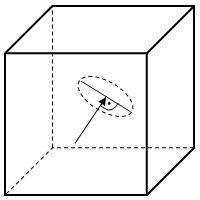
\includegraphics{pics/Vektor-Orthogonalitaet.jpg}
  %%   \caption{Unendlich viele Vektoren}
  %% \end{figure}
\item Es entsteht eine Ebene, die orthogonal zum Ausgangsvektor
  liegt. Sind die Vektoren alle gleich lang, so enteht ein Kreis,
  dessen Mittelpunkt der nicht verschobene Punkt ist und dessen
  Radius gleich der Länge der Vektoren ist.
\item Man vertauscht zwei Koordinaten und ändert bei einer das
  Vorzeichen. Die dritte Koordinate wird auf 0 gesetzt.
  \begin{multicols}{4}
    \begin{enumerate}
    \item $  
      \begin{pmatrix}
        1\\0\\0
      \end{pmatrix}
      $
    \item $  
      \begin{pmatrix}
        1\\-1\\0
      \end{pmatrix}
      $
    \item $  
      \begin{pmatrix}
        -4\\0\\3
      \end{pmatrix}
      $
    \item $  
      \begin{pmatrix}
        1\\0\\-7
      \end{pmatrix}
      $
    \end{enumerate}
  \end{multicols}
\item Sie sind alle paarweise zueinander orthogonal, da sie alle eine
  jeweils andere Koordinate haben, die nicht 0 ist. (Sie sind jeweils parallel
  zu einer Koordinatenachse)
\end{enumerate}
\subsection{Vektoren auf Orthogonalität prüfen}
  \begin{enumerate}
  \item \textbf{Beispiel: d)}
    $ \Vektor{-7}{2}	\perp	\Vektor{-2}{-7}	\Leftrightarrow	(-7)\cdot(-2)+2\cdot(-7)	=+14-14	= 0 $ \\
    $ \Vektor{-7}{2}	\perp	\Vektor{2}{7}	\Leftrightarrow	(-7)\cdot2 + 2\cdot7		=-14+14	= 0 $
		
  \item
    \begin{multicols}{2}
    \item[\textbf{a.)}]
      $ 2\cdot(-6)+1\cdot12=0 \Leftrightarrow \Vektor{2}{1} \perp \Vektor{-6}{12}$\newline
    \item[\textbf{b.)}]
      $ 14\cdot4+(-8)\cdot7=0 \Leftrightarrow \Vektor{14}{4} \perp \Vektor{-8}{7}$\newline
    \item[\textbf{c.)}]
      $ (-1)\cdot4+(-4)\cdot1=-8 \Leftrightarrow \Vektor{2}{1} \not \perp \Vektor{-6}{12}$\newline
    \item[\textbf{d.)}]
      $ 7\cdot1+2\cdot(-3,5)=0 \Leftrightarrow \Vektor{7}{2} \perp \Vektor{1}{-3,5}$
    \end{multicols}
    
    
  \item
	Wir übernehmen den Satz des Pythagoras von oben: 
		$$|\vec{a}|^2 + |\vec{b}|^2 = |\vec{b} - \vec{a}|^2 $$
	und setzen die Vektoren ein:
		$$ \begin{array}{|c|}	\vektor{a_{1}}{a_{2}}{a_{3}} \end{array} ^2 + \begin{array}{|c|}\vektor{b_{1}}{b_{2}}{b_{3}} \end{array} ^2 = \begin{array}{|c|} \vektor{b_{1}}{b_{2}}{b_{3}} -	\vektor{a_{1}}{a_{2}}{a_{3}}\end{array} ^2  $$
	Wir beginnen mit den Rechenschritten um die Betragsstriche aufzulösen:
		$$ \sqrt{(a_1)^{2} + (a_{2})^2 + (a_{3})^2} ^2 + \sqrt{(b_1)^{2} + (b_{2})^2 + (b_{3})^2} ^2 = \sqrt{(b_1-a_1)^2 + (b_2-a_2)^2 + (b_3-a_3)^2}^2 $$
		Die $\sqrt{}$ können wir aufgrund des $^2$ einfach eliminieren und dann mithilfe der zweiten Binomischen Formel die Klammern rechts auflösen:
		$$ (a_1)^{2} + (a_2)^2 + (a_3)^2 + (b_1)^{2} + (b_2)^2 + (b_3)^2 = $$
		$$ (b_1)^2 - 2b_{1}a_{1} + (a_1)^2 + (b_2)^2 - 2b_{2}a_{2} + (a_2)^2 + (b_3)^2 - 2b_{3}a_{3} + (a_3)^2	$$
	Nun Streichen wir alles, was auf beiden Seiten vorkommt:
		$$ \cancel{(a_1)^{2}} + \cancel{(a_2)^2} + \cancel{(a_3)^2} + \cancel{(b_1)^2} + \cancel{(b_2)^2} + \cancel{(b_3)^2} =$$
		$$ \cancel{(b_1)^2} - 2b_{1}a_{1} + \cancel{(a_1)^2} + \cancel{(b_2)^2} - 2b_{2}a_{2} + \cancel{(a_2)^2} + \cancel{(b_3)^2} - 2b_{3}a_{3} + \cancel{(a_3)^2} $$
	Übrig bleibt:
		$$ 0 = 	- 2b_{1}a_{1} - 2b_{2}a_{2} - 2b_{3}a_{3} $$
	Wir teilen auf beiden Seiten der Gleichung durch -2 und erhalten: 
		$$ 0 = b_{1}a_{1} + b_{2}a_{2} + b_{3}a_{3} $$

		\item Wir benutzen unsere Erkenntnis aus \textbf{3.)} und setzen die Zahlen aus den Vektoren in die Gleichung ein. Wenn 0 heraus kommt, müssen die Vektoren orthogonal sein.
			\begin{multicols}{2}
				\item[\textbf{a.)}] 	$ 1\cdot0 + 1\cdot0 + 1\cdot0 = 0 $ 	\\ Also sind die Vektoren orthogonal.
				\item[\textbf{b.)}] 	$ 2\cdot(-4)+3\cdot0+4\cdot2=-8+8= 0$ 	\\ Also sind die Vektoren orthogonal.
				\item[\textbf{c.)}] 	$ 1\cdot2+2\cdot2+3\cdot(-2)=2+4-6=0$ 	\\ Also sind die Vektoren orthogonal.
				\item[\textbf{d.)}] 	$0\cdot0+0\cdot(-1)+2\cdot1=2$ 		\\ Also sind die Vektoren \underline{nicht} orthogonal.
			\end{multicols}
		
		
		\item
		Wir setzen jeweils in die Gleichung aus \textbf{3.)} ein und lösen nach a auf:
		\item[\textbf{a.)}] 
		\begin{align*}
			3\cdot(-1) + 4\cdot2 + 1\cdot a &= 0 \\
			-3 + 8 + a &= 0 	\qquad | +3 -8  \\
			\uu{a = -5}
		\end{align*}
		\item[\textbf{b.)}] 
		\begin{align*}
			7\cdot1+1\cdot a+5\cdot2&=0\\
			7+a+10&=0 			\qquad |-17\\
			\uu{a=-17}
		\end{align*}
		\item[\textbf{c.)}]
		\begin{align*}
				10\cdot a+27\cdot1+0,5\cdot(-14)&=0\\
			10a+27-7&=0 		\qquad |-20\quad |:10\\
			\uu{a=-2}
		\end{align*}
              \item[\textbf{d.)}] 
		\begin{align*}
			8\cdot2+3\cdot a+1\cdot a &=0 \\
			16+4a &=0 			\qquad |-16 \quad |:4\\
			\uu{a=-4}
		\end{align*}
	\end{enumerate}
	
\section{Skalarprodukt}
	\subsection{Skalarprodukt und Orthogonalität}	 
	\begin{enumerate}
 		\item \hfill
 			\begin{multicols}{2}
 				\item[\textbf{a.)}] $$ \Vektor{5}{0} 		\cdot \Vektor{1}{3} 	= 5\cdot1+0\cdot3=5  $$
 				\item[\textbf{b.)}]	$$ \vektor{1}{3}{1} 	\cdot \vektor{2}{5}{1} 	= 1\cdot2+3\cdot5+1\cdot1=18 $$
 				\item[\textbf{c.)}]	$$ \vektor{1}{3}{5}		\cdot \vektor{5}{3}{1} 	= 1\cdot5+3\cdot3+5\cdot1=19 $$
 				\item[\textbf{d.)}]	$$ \vektor{-11}{4}{1} 	\cdot \vektor{1}{2}{3} 	= (-11)\cdot1+4\cdot2+1\cdot3=0 $$
 			\end{multicols}
 		
 		\item Um zu überprüfen, ob die beiden Geraden orthogonal sind, genügt es uns, die Richtungsvektoren zu überprüfen. Wenn diese orthogonal zueinander liegen, tut das die ganze Gerade.
 		$$ \vektor{-5}{1}{0} \cdot \vektor{-2}{2}{0} = (-5)\cdot(-2)+1\cdot2+0\cdot0=10+2=12 \not = 0 \Leftrightarrow \vektor{-5}{1}{0} \not \perp \vektor{-2}{2}{0} $$ 		
 		
 		\item Hier denken wir uns einen unvollständigen Vektor aus, den wir als Richtungsvektor für die Gerade h nehmen. Der Einfachhalt halber hier: $\vektor{1}{1}{a}$.
 		Dann suchen wir a unter der Voraussetzung, dass der Vektor orthogonal zum Richtungsvektor von g ist.
 			\begin{multicols}{2}
	 			\item[\textbf{a.)}] $$ \vektor{7}{17}{-2} \perp \vektor{1}{1}{a} \Leftrightarrow  7\cdot1 + 17\cdot1 + (-2)\cdot a = 0 $$
 									$$7+17-2a=0 \qquad |-24 \quad |:(-2)$$
 									$$\uu{a=12}$$
 									$$\vektor{7}{17}{-2} \perp \vektor{1}{1}{12}$$
 				\item[\textbf{b.)}]	$$ \vektor{1}{2}{-3} \perp 				\vektor{1}{1}{a} \Leftrightarrow 1\cdot1 + 2\cdot1 + (-3)\cdot a = 0 $$
 									$$1+2-3a=0 \qquad |-3 \quad |:(-3)$$
 									$$\uu{a=1}$$
									$$\vektor{1}{2}{-3} \perp \vektor{1}{1}{1}$$
	 		\end{multicols}
 			
	 	\item Wir müssen jeweils Überprüfen, ob $\vec{AB}$, $\vec{BC}$ und $\vec{CA}$ orthogonal sind.
			\begin{multicols}{2}
				\item[\textbf{a.)}]	
							$\vec{AB}  = \vektor{3}{1}{4} $ 
				\item[]		$\vec{BC}  = \vektor{-1}{-3}{-5} $  	
				\item[]		$\vec{CA}  = \vektor{-2}{2}{1} $
 				\item[] 	$\vec{AB} \cdot \vec{BC} = \vektor{3}{1}{4} 	\cdot \vektor{-1}{-3}{-5} 	= -3-3-20 \not= 0 $ 
 				\item[]		$\vec{BC} \cdot \vec{CA} = \vektor{-1}{-3}{-5} 	\cdot \vektor{-2}{2}{1} 	= 2-6-5 \not= 0 $
 				\item[] 	$\vec{CA} \cdot \vec{AB} = \vektor{-2}{2}{1} 	\cdot \vektor{3}{1}{4} 		= -6 +2 +4 = 0$ 
 				\item[]
				\item[$\Leftrightarrow$]	
   							$\vec{CA} \perp \vec{AB} $
 			\end{multicols}		
 		
\bigskip	
			\begin{multicols}{2}
				\item[\textbf{b.)}]	
						$\vec{AB}  = \vektor{1}{-3}{-1} $ 
				\item[]	$\vec{BC}  = \vektor{-5}{-3}{4} $ 
				\item[]	$\vec{AB} \cdot \vec{BC} = \vektor{1}{-3}{-1} 	\cdot \vektor{-5}{-3}{4} 	=$ \\ $ 1\cdot(-5) + (-3)\cdot(-3) + (-1)\cdot4 = $\\$-5+9-4 = 0 $ 
	 			\item[$\Leftrightarrow$] $\vec{CA} \perp \vec{AB}$
 			\end{multicols}
	\item
%Wir suchen einen Vektor, für den die Gleichung aus 3.) für beide Vektoren gilt: \\
%			$$\vektor{1}{2}{3} \cdot \vektor{x}{y}{z} =0 \hspace{3cm} \vektor{2}{0}{3} \cdot \vektor{x}{y}{z} =0  $$
%		Wir rechnen das Skalarprodukt aus und erhalten zwei Gleichungen eines Gleichungssystems:
%			$$ \begin{array}{rrrr}
% 			1x&+2y&+3z &= 0 \\
%			2x&&+3z&=0 
%			\end{array}$$
%		Da wir drei Unbekannte aber nur zwei Gleichungen haben, können wir 	

		\item Wir müssen alles Winkel auf Orthogonalität überprüfen oder bis wir ein Gegenbeweis gefunden haben.
			\setlength{\columnsep}{-5cm}
			\begin{multicols}{2}
				\item[\textbf{a.)}]	
						$\vec{AB}  = \vektor{-1}{-2}{-1} $ 
				\item[]	$\vec{BC}  = \vektor{-11}{1}{9} $  	
				\item[]	$\vec{CD}  = \vektor{1}{2}{1} $
				\item[] $\vec{DA}  = \vektor{11}{-1}{-9} $
				\item[] $\vec{AB} \cdot \vec{BC} = \vektor{-1}{-2}{-1} 	\cdot \vektor{-11}{1}{9} 	= 11-2-9 = 0 $ 
				\item[]	$\vec{BC} \cdot \vec{CD} = \vektor{-11}{1}{9} 	\cdot \vektor{1}{2}{1} 		= -11+2+9 = 0 $
				\item[]	$\vec{CD} \cdot \vec{DA} = \vektor{1}{2}{1} 	\cdot \vektor{11}{-1}{-9} 	= 11-1-9 = 0 $
				\item[] $\vec{DA} \cdot \vec{AB} = \vektor{11}{-1}{-9} 	\cdot \vektor{-1}{-2}{-1} 	= -11+2+9 = 0$ 
 			\end{multicols}
\medskip
 			\setlength{\columnsep}{-5cm}
 			\begin{multicols}{2}
 				\item[\textbf{b.)}]	
 						$\vec{AB}  = \vektor{-1}{-1}{7} $ 
 				\item[]	$\vec{BC}  = \vektor{-5}{8}{-1} $  	
 				\item[] $\vec{AB} \cdot \vec{BC} = \vektor{-1}{-1}{7} 	\cdot \vektor{-5}{8}{-1} 	= 5-8-7 \not= 0 $ 
 				\item[]	$\Leftrightarrow \vec{AB} \not\perp \vec{BC}$
 			\end{multicols}
\medskip
 			\setlength{\columnsep}{-5cm}
 			\begin{multicols}{2}
 				\item[\textbf{7.)}]	$\vec{AC}  = \Vektor{5}{5} $ 
 				\item[]	$\vec{BD}  = \Vektor{3}{-3} $  	
 				\item[] $\vec{AC} \cdot \vec{BD} = \Vektor{5}{5} 	\cdot \Vektor{3}{-3} 	= 15-15 = 0 $ 
 				\item[]	$\Leftrightarrow \vec{AC} \perp \vec{BD}$
 			\end{multicols}
 	\end{enumerate}
\subsection{Winkelberechnung mithilfe des Skalarprodukts}
	\begin{enumerate}
		\item Da $\cos(90^\circ)=0$ kommt bei einem rechten Winkel mit der Gleichung $\vec{a}\cdot\vec{b}=|\vec{a}|\cdot|\vec{b}|\cdot0 $ stets Null raus. Demnach ist $\vec{a}\cdot\vec{b} = 0$ stets ein Zeichen für Orthogonalität.

		\item * Wir beginnen mit dem Kosinussatz, geben ihm Vektoren-Einheiten und formen um:
		
		{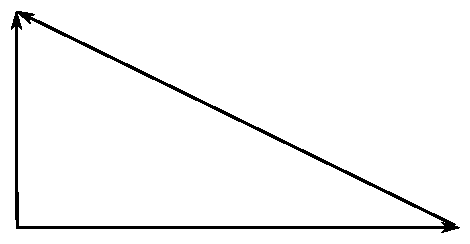
\includegraphics [keepaspectratio,height=5cm]{pics/Dreieck}}
		$$a=\vec{AB}=\vektor{a_1}{a_2}{a_3}$$			$$b=\vec{BC}=\vektor{b_1}{b_2}{b_3}$$
		$$c=\vec{CA}=\vektor{c_1}{c_2}{c_3}$$\newline\newline
Wir nehmen den Kosinussatz:				
		$$ a^2=b^2+c^2-2ab\cdot cos(\alpha)$$
Dort setzten wir die Bezeichnungen in Vektoren-Schreibweise hinein:	
		$$ |\vec{BC}|^2=|\vec{CA}^2|+|\vec{AB}|^2-2|\vec{CA}||\vec{AB}|\cdot cos(\alpha) $$
Wir tauschen $\vec{BC}$ mit $\vec{CA-AB}$ um nur noch zwei statt drei unterschiedlicher Vektoren zu haben:	
		$$|\vec{CA}-\vec{AB}|^2=|\vec{CA}|^2+|\vec{AB}|^2-2|\vec{CA}||\vec{AB}|\cdot cos(\alpha) \qquad |-|\vec{CA}|^2-|\vec{AB}|^2 $$
Dann fangen wir an die Formel nach $\alpha$ umzustellen:	
		$$|\vec{CA}-\vec{AB}|^2-|\vec{CA}|^2-|\vec{AB}|^2=-2|\vec{CA}||\vec{AB}|\cdot \cos(\alpha) $$
Wir schreiben die Vektoren ganz auf,	
		$$\left|\vektor{c_1-a_1}{c_2-a_2}{c_3-a_3}\right|^2-\left|\vektor{c_1}{c_2}{c_3}\right|^2-\left|\vektor{a_1}{a_2}{a_3}\right|^2=-2|\vec{CA}||\vec{AB}| \cdot \cos(\alpha) $$
um sie dann besser auseinanderziehen zu können:	
		$$\sqrt{(c_1-a_1)^2+(c_2-a_2)^2+(c_3-a_3)^2}^2-\sqrt{{c_1}^2+{c_2}^2+{c_3}^2}^2-\sqrt{{a_1}^2+{a_2}^2+{a_3}^2}^2=$$
		$$-2|\vec{CA}||\vec{AB}|\cdot \cos(\alpha) $$
Die Wurzeln und die Quadrate eliminieren sich:	
		$$(c_1-a_1)^2+(c_2-a_2)^2+(c_3-a_3)^2-{c_1}^2+{c_2}^2+{c_3}^2-{a_1}^2+{a_2}^2+{a_3}^2=$$
		$$-2|\vec{CA}||\vec{AB}|\cdot \cos(\alpha) $$
Und nach dem Anwenden der 2. Binomischen Formel eliminiert sich einiges in der Formel selbst:		
		$$\cancel{{c_1}^2}-2c_1a_1+\cancel{{a_1}^2}\quad+\quad\cancel{{c_2}^2}+-c_2+a_2+\cancel{{a_2}^2}\quad+\quad\cancel{{c_3}^2}-2c_3+a_3+\cancel{{a_3}^2}\quad-\cancel{{c_1}^2}+\cancel{{c_2}^2}+\cancel{{c_3}^2}-\cancel{{a_1}^2}+\cancel{{a_2}^2}+\cancel{{a_3}^2}=$$
		$$-2|\vec{CA}||\vec{AB}|\cdot \cos(\alpha) $$
Jetzt ziehen wir noch den Rest der rechten Seite auf die Linke, um $\cos(\alpha)$ alleine zu haben:
		$$-2c_1a_1-2c_2a_2-2c_3a_3=-2|\vec{CA}||\vec{AB}|\cdot \cos(\alpha) \qquad | :-2|\vec{CA}||\vec{AB}|$$
Als letztes Kürzen wir mit $-2$ und können aus dem Rest oberhalb des Bruches wieder zwei Vektoren bilden ($\vec{a}\cdot\vec{c}=a_1c_1+a_2c_2+a_3c_3$):	
		$$\dfrac{\cancel{-2}c_1a_1+\cancel{-2}c_2a_2+\cancel{-2}c_3a_3}{\cancel{-2}|\vec{CA}||\vec{AB}|}=\dfrac{c_1a_1+c_2a_2+c_3a_3}{|\vec{CA}||\vec{AB}|}=\dfrac{\vec{CA}\cdot\vec{AB}}{|\vec{CA}||\vec{AB}|}=\cos(\alpha)$$
	

	
		\item
			\begin{enumerate}
				\item[\textbf{a.)}]	$$ \cos(\alpha)=\dfrac{\Vektor{5}{0} \cdot \Vektor{1}{3}} {\left|\Vektor{5}{0}\right| \cdot \left| \Vektor{1}{3}\right|}=\dfrac{5\cdot1+3\cdot0} {\sqrt{5^2} \cdot \sqrt{3^2+1^2}} $$
								
				$$ \cos(\alpha)=\dfrac{\cancel{5}}{\cancel{5}\cdot\sqrt{10}} \qquad \left|\cos{}^{-1}\right.$$ 
								
				$$\alpha=\cos^{-1}\left(\dfrac{1}{\sqrt{10}}\right)$$
				
				$$\uu{\alpha = 71\mathrm{,}57^\circ}$$
\medskip
				\item[\textbf{b.)}]			
				$$\alpha=\cos^{-1}\left(\cfrac{2+15+1}{\sqrt{1+9+1}\cdot\sqrt{4+25+1}}\right)=\cos^{-1}\left(\cfrac{18}{\sqrt{11}\cdot\sqrt{30}}\right)=7\mathrm{,}75^\circ$$
				\item[\textbf{c.)}]	$$\alpha=\cos^{-1}\left(\cfrac{5+9+5}{\sqrt{1+9+25}\cdot\sqrt{25+9+1}}\right)=\cos^{-1}\left(\cfrac{19}{\sqrt{35}\cdot\sqrt{35}}\right)=57\mathrm{,}12^\circ$$
				\item[\textbf{d.)}]	$$\alpha=\cos^{-1}\left(\cfrac{-11+8+3}{\sqrt{144+16+1}\cdot\sqrt{1+4+9}}\right)=\cos^{-1}\left(\cfrac{0}{\sqrt{161}\cdot\sqrt{14}}\right)=90^\circ$$	
		\end{enumerate}
		\hfill\newline
		\end{enumerate}
%Neuaufsetzung wegen komischen Einschubs		
		\begin{enumerate}
		\setcounter{enumi}{3}
		\item 
		\begin{enumerate}
			\item	$\vec{AB}=\Vektor{3}{-2} \qquad \vec{BC}=\Vektor{-1}{4} \qquad \vec{CA}=\Vektor{-2}{-2}$
			\bigskip\newline
			$  a=|\vec{BC}| = \left|\Vektor{-1}{4}\right| = \sqrt{(-1)^2+4^2} = \sqrt{1+16} = \sqrt{17}\\ b=|\vec{CA}|=\left|\Vektor{-2}{-2}\right| = \sqrt{(-2)^2+(-2)^2} = \sqrt{4+4}=\sqrt{8}\\ 
			c=|\vec{AB}| = \left|\Vektor{3}{-2}\right| = \sqrt{3^2+(-2)^2} = \sqrt{9+4} =\sqrt{13}$\\
			\bigskip\newline
			$ \alpha = cos^{-1} \left(\frac{\vec{AB} \cdot
                            \vec{AC}}{|\vec{AB}|\cdot |AC|}\right)
                        = cos^{-1} \left(\frac{6-4}{\sqrt{13} \cdot \sqrt{8}}\right)
                        = 78,69^\circ $\\
			$ \beta = cos^{-1}
                        \left(\frac{\vec{BA}\cdot\vec{BC}}{|\vec{BA}|\cdot|BC|}\right)
                        =cos^{-1}
                        \left(\frac{3+8}{\sqrt{13}\cdot\sqrt{17}}\right)
                        =42,27^\circ$\\
			$ \gamma = cos^{-1}
                        \left(\frac{\vec{CB}\cdot\vec{CA}}{|\vec{CB}|\cdot|CA|}\right)
                        =cos^{-1} \left(\frac{8-2}{\sqrt{17}\cdot\sqrt{8}}\right) =59,04^\circ $
			
			\item 
			$c= |\vec{AB}|=\left|\Vektor{ 8}{-3} \right|=\sqrt{73}\\
			 a= |\vec{BC}|=\left|\Vektor{-6}{10}\right|=\sqrt{136}\\
			 b= |\vec{CA}|=\left|\Vektor{-2}{-7}\right|=\sqrt{53}$
			 
			$\alpha=46,91^\circ\\
			 \beta=38,48^\circ\\
			 \gamma=94,61^\circ$
			
			\item
			$|\vec{AB}|=\sqrt{20}
			 |\vec{BC}|=\sqrt{20}
			 |\vec{CA}|=\sqrt{32}$
			 
			 $\alpha=46,91^\circ\\
			 \beta=38,48^\circ\\
			 \gamma=94,61^\circ$
			 \item
		\end{enumerate}
		
		\bigskip
		\item 	
		\begin{enumerate}									
			\item	$\cos(30) =\dfrac{\vektor{0}{1}{0} \cdot \vektor{\sqrt{3}}{b}{0}} {\left|\vektor{0}{1}{0}\right| \cdot \left|\vektor{\sqrt{3}}{b}{0}\right|} = \dfrac{b}{\sqrt{3+b^2}}      \qquad \left|\cdot \sqrt{3+b^2}\right.$\\
			
			\begin{align*}
			\cos(30) \cdot \sqrt{3+b^2} = b &	\umf{^2} \\			
			\cos(30)^2 \cdot (3+b^2) = b^2&\\			
			\cos(30)^2 \cdot 3 + \cos(30)^2 \cdot b^2 = b^2      &\umf{\-b^2\cdot cos(30)^2}\\			
			\cos(30)^2 \cdot 3 = 1 \cdot b^2 - (\cos(30)^2 \cdot b^2)\\			
			\cos(30)^2 \cdot 3 = b^2 \cdot (1-cos(30)^2) &\umf{:(1-cos(30))}\\		
			\dfrac{\cos(30)^2 \cdot 3}{1-cos(30)^2}=b^2 &\umf{\sqrt{~}}\\			
			\dfrac{\sqrt{\cos(30)^2 \cdot 3}}{\sqrt{1-cos(30)^2}}=b\\			
			\uu{\pm3=b}
			\end{align*}
                      \item

                        Wir setzen eine Gleichung über die Winkel-Formel an:
                        $$\cos(60)=
                        \frac{\vektor{0}{0,5}{0,5} \cdot \vektor{1}{0}{c}}
                        {\left|\vektor{0}{0,5}{0,5}\right| \cdot
                          \left|\vektor{1}{0}{c}\right|}$$

                        Wir setzen $\cos(60)=0,5$ ein, berechnen das
                        Skalarprodukt und die Längen und setzen alles ein.
                        Wenn die Unbekannte im Nenner steht,
                        müssen wir die Gleichung mit dem Nenner
                        multiplizieren:
                        \begin{align*}
                          0,5 &=\frac {0,5\cdot c}
                                {\sqrt{0,5}\cdot\sqrt{1+c^2}}&|\quad
                                                                 \cdot
                                                                 \sqrt{0,5}\cdot\sqrt{1+c^2}&\\
                          0,5\cdot \sqrt{0,5}\cdot\sqrt{1+c^2}
                              &=0,5\cdot c &|\quad \cdot 2&\\
                          \sqrt{0,5}\cdot\sqrt{1+c^2}&=c &\quad \textrm{alles
                                                           quadrieren, damit
                                                           die Wurzel
                                                           wegkommt}&\\
                          0,5\cdot (1+c^2) &= c^2& &\\
                          0,5 +0,5c^2 &= c^2 &\quad | -0,5c^2 &\\
                          0,5 &= 0,5c^2 & \quad | \cdot 2 &\\
                          1&= c^2 &\quad |\sqrt{ } &\\
                          c&=1
                        \end{align*}
                        Da wir einmal alles quadriert haben, ist die
                        negative Lösung ausgeschlossen.

                        
		\end{enumerate}			
		
		\item
		\begin{align*}
			&&\sphericalangle \vec{a}, \vec{b}   &=45^\circ\\
			&&\sphericalangle \vec{-a}, \vec{b}  &=135^\circ\\
			&&\sphericalangle \vec{a} , \vec{-b} &=135^\circ\\
			&&\sphericalangle \vec{-a}, \vec{-b} &=45^\circ\\
		\end{align*}
		
		\item
		Wenn das Skalarprodukt negativ ist, ist der ganze Bruch negativ. Dann geben wir $cos^{-1}$ eine negative Zahl. 
		\begin{align*}
		cos^{-1}(1)		&= 0\\
		cos^{-1}(0,5)	&= 60\\
		cos^{-1}(0)		&= 90\\
		cos^{-1}(-0,5)	&= 120\\
		cos^{-1}(-1)	&= 180\\
		\end{align*}
		Wenn das Skalarprodukt negativ ist, scheint der Winkel größer als $90^\circ$ zu sein.
		
		\item %? 
		
		\item %M ist Schnittpunkt der Raumdiagonalen mit was?
	\end{enumerate}
	
\section{Vektorprodukt}
	\begin{enumerate}
\item
	\begin{enumerate}
		\item $\vec{a} \times \vec{b} = \vektor{1}{2}{3}\times\vektor{4}{5}{6}=\vektor{2 \cdot 6 - 3 \cdot 5}{3 \cdot 4 - 1 \cdot 6}{1 \cdot 5 - 2 \cdot 4} =\vektor{-3}{6}{-3}$
		\item $\vektor{1}{2}{0}\times\vektor{3}{1}{0}=\vektor{0}{0}{-5}$
		\item $\vektor{-4}{3}{0}\times\vektor{2}{-9}{-1}=\vektor{-3}{-4}{30}$
		\item $\vektor{0}{1}{-3}\times\vektor{8}{-8}{5}= \vektor{-19}{-24}{-8}$
	\end{enumerate}

\item
	\begin{enumerate}
		\item 1b:	$\vektor{3}{1}{0}\times\vektor{1}{2}{0}=\vektor{0}{0}{-5}$\\
			  1c:	$\vektor{2}{-9}{-1}\times\vektor{-4}{3}{0}=\vektor{-3}{-4}{30}$\\
			  Schlussfolgerung: $\vec{a}\times\vec{b}=\vec{b}\times\vec{a}$\bigskip
		\item 1b:	$\vektor{1}{2}{0}\cdot\left(\vektor{1}{2}{0}\times\vektor{3}{1}{0}\right)=0$\\
			  1c:	$\vektor{-4}{3}{0}\cdot\left(\vektor{-4}{3}{0}\times\vektor{2}{-9}{-1}\right)=0$\\
			  Schlussfolgerung: $\vec{a}\cdot(\vec{a}\times\vec{b})=0$\bigskip
		\item Da nach a) $$\vec{b}\cdot(\vec{a}\times\vec{b})=\vec{b}\cdot(\vec{b}\times\vec{a}),$$ geschieht hier dasselbe wie bei b).\\		
	\end{enumerate}
	UND: Da $\vec{a}\cdot(\vec{a}\times\vec{b})=0$, ist $$\vec{a}\perp\vec{a}\times\vec{b}$$
	
\end{enumerate}

\end{document}


